\subsection{Prediction of visual features}
\label{subsec:visual}
The models are trained and evaluated on the prediction of visual feature vectors from captions. We are not devising an image retrieval method, but this task reflects the ability to extract visually salient semantic information from language.
For the experiments on the prediction of visual features all models
were trained on the training set of MS COCO. As validation and test data we
used a random sample of 5000 images each from the MS COCO validation set. 

Figure~\ref{fig:loss} shows the value of the validation average cosine distance
between the predicted visual vector and the target vector for three
random initializations of each of the model types. 

The Phonetic GRU model is more sensitive to the initialization: one
can clearly distinguish three separate trajectories. The word-level models
are much less affected by random initialization. In terms of the
overall performance, the {\sc Phon GRU} model falls between the
{\sc Word Sum} model and the {\sc Word GRU} model.

\begin{figure}
    \centering
  \begin{minipage}{0.45\textwidth}
    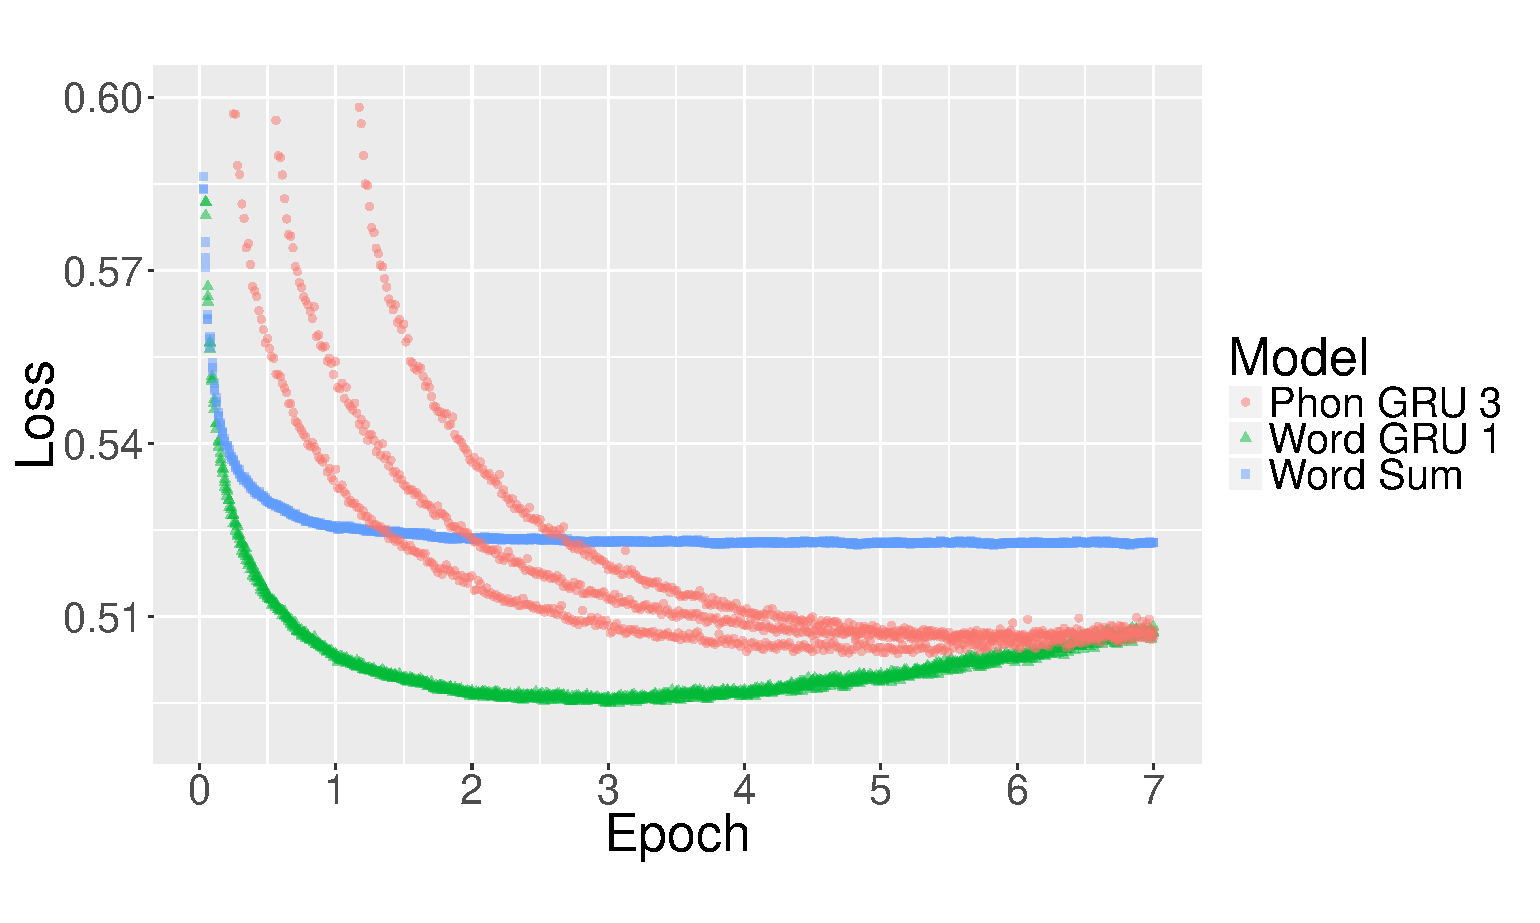
\includegraphics[scale=0.3]{loss-zoom.pdf}
    \caption{Value of the loss function on validation data during
      training. Three random initialization of each model are shown.}
    \label{fig:loss}
  \end{minipage}
\hspace{0.3cm}
  \begin{minipage}{0.45\textwidth}
    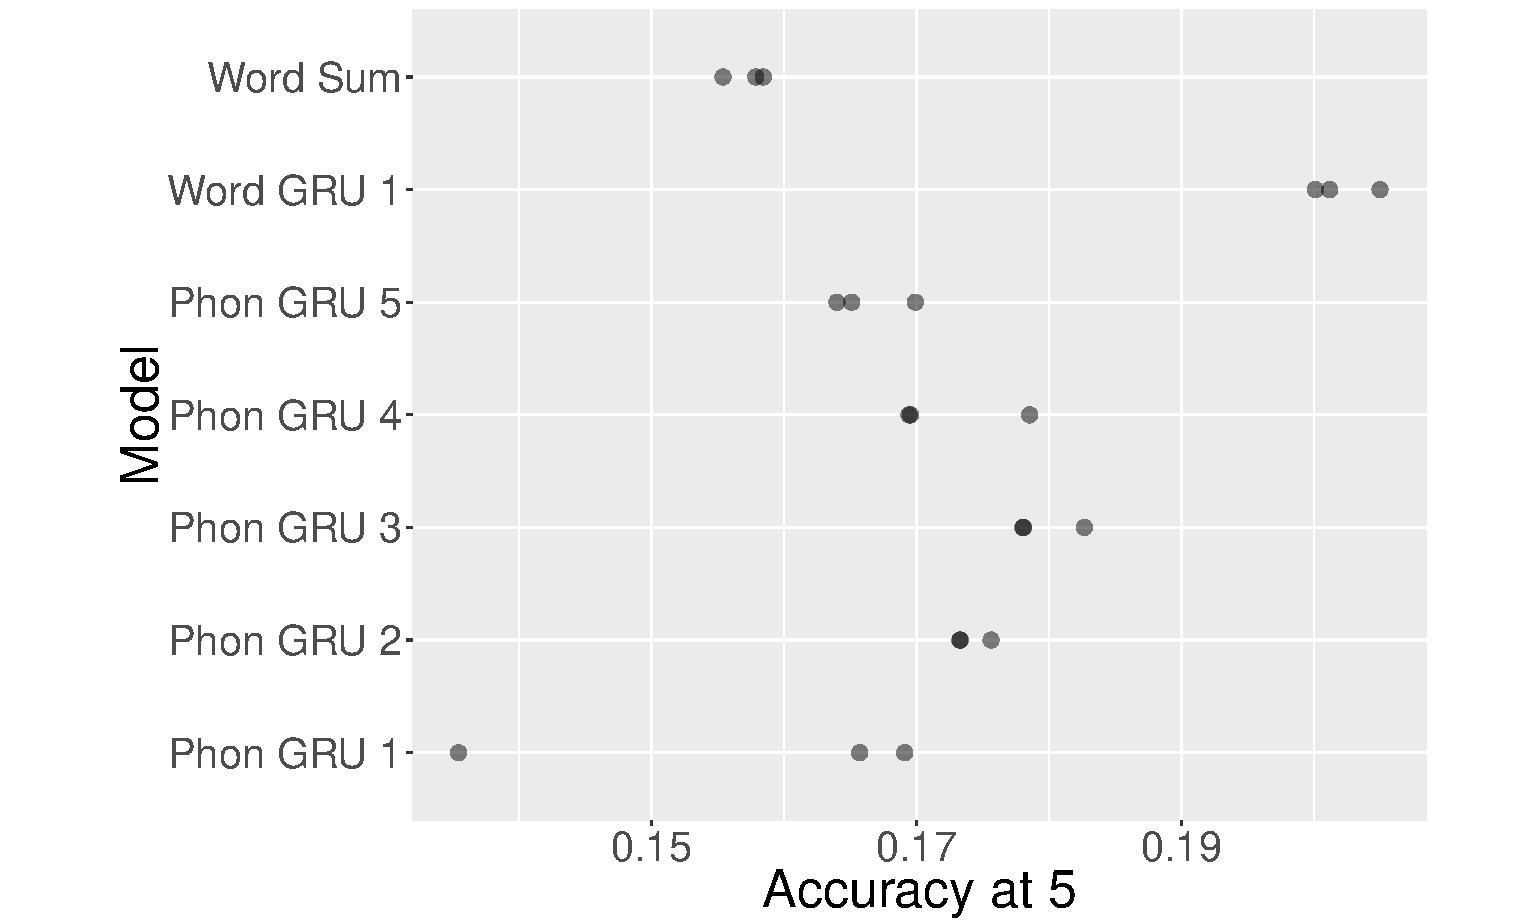
\includegraphics[scale=0.25]{accat5.pdf}
    \caption{Validation accuracy at 5 on the image retrieval task.}
    \label{fig:accat5}
  \end{minipage}
\end{figure}

We also evaluated the models on how well they perform when used to
search images: for each validation sentence the model was used to predict the
visual vector. The image vectors in the validation data were then
ranked by cosine similarity to the predicted vector, and the
proportion of times the correct image was among the top 5 was
reported. By {\it correct} image we mean the one which the sentence
was used to describe (even though often many other images are also
good matches to the sentence). 

In Figure~\ref{fig:accat5} we report the validation accuracies on this
task for the two word-level models, as well as for the Phon GRU
model with different number of hidden layers. We trained each model
version with three random initializations for each model setting, and
evaluate after each epoch. We report the score of the best epoch for
each initialization. 
The overall ranking of the models matches the direct
evaluation of the loss function above: the phoneme-level models are in
between the two word-level models. {\sc Phon GRU} with three
hidden layers is the best of the phoneme-level models.

In Table~\ref{tab:accat5test} we show the accuracies of the best
version of each of the models types on the test images; these are also
the model versions used in all subsequent experiments. The accuracy @ 5 for the {\sc Word GRU} is comparable to what
\newcite{chrupala2015learning} report for their multitask {\sc Imaginet}
model, whose visual pathway has the same structure.


% \begin{table}
%   \centering
%   \begin{tabular}{ll|r}
%  Model     & Layers & Acc. at 5 \\\hline
%  Word Sum  & 0      & 0.158 \\
%  Word GRU  & 1      & 0.205 \\\hline
%  Phon GRU  & 1      & 0.169  \\
%  Phon GRU  & 2      & 0.176  \\
%  Phon GRU  & 3      & \bf 0.183  \\  
%  Phon GRU  & 4      & 0.179 \\
%  Phon GRU  & 5      & 0.170 \\
%   \end{tabular}
% \caption{Accuracy at 5 on the image retrieval task.}
% \label{tab:accat5}
% \end{table}
